\documentclass[11pt,a4paper]{article}

%% ── Packages ─────────────────────────────────────────────────
\usepackage[a4paper,top=24mm,bottom=24mm,left=22mm,right=22mm]{geometry}
\usepackage[T1]{fontenc}
\usepackage[protrusion=false,expansion=false]{microtype}
\usepackage{booktabs}
\usepackage{longtable}
\usepackage{array}
\usepackage{tabularx}
\usepackage{multirow}
\usepackage{xcolor}
\usepackage{colortbl}
\usepackage{amsmath}
\usepackage{enumitem}
\usepackage{fancyhdr}
\usepackage{titlesec}
\usepackage{parskip}
\usepackage{mdframed}
\usepackage{hyperref}
\usepackage{tikz}
\usepackage{pgfplots}
\pgfplotsset{compat=1.18}
\usetikzlibrary{arrows.meta,positioning,shapes.geometric,fit,
                backgrounds,calc,shadows.blur}

%% ── Colours ──────────────────────────────────────────────────
\definecolor{ddrblue}  {RGB}{20, 80,150}
\definecolor{ddrteal}  {RGB}{0, 115,105}
\definecolor{ddramber} {RGB}{185,115,  0}
\definecolor{ddrgreen} {RGB}{0, 120, 65}
\definecolor{ddrred}   {RGB}{165, 25, 25}
\definecolor{ddrpurple}{RGB}{95,  35,135}
\definecolor{lightgray}{RGB}{247,247,247}
\definecolor{rowblue}  {RGB}{233,243,255}
\definecolor{rowgreen} {RGB}{233,250,240}
\definecolor{roworange}{RGB}{255,245,228}
\definecolor{rowred}   {RGB}{255,237,237}
\definecolor{rowpurple}{RGB}{245,235,255}
\definecolor{rowteal}  {RGB}{229,249,247}
\definecolor{rowgray}  {RGB}{245,245,245}

%% ── Hyperref ─────────────────────────────────────────────────
\hypersetup{colorlinks=true,linkcolor=ddrblue,urlcolor=ddrteal,
            pdftitle={MC Core Design Specification}}

%% ── Section style ────────────────────────────────────────────
\titleformat{\section}
  {\large\bfseries\color{ddrblue}}{}{0em}{}[\color{ddrblue}\titlerule]
\titleformat{\subsection}
  {\normalsize\bfseries\color{ddrteal}}{}{0em}{}
\titleformat{\subsubsection}
  {\normalsize\bfseries\color{ddramber}}{}{0em}{}

%% ── Header / Footer ──────────────────────────────────────────
\pagestyle{fancy}\fancyhf{}
\renewcommand{\headrulewidth}{0.4pt}
\fancyhead[L]{\small\textcolor{ddrblue}{\textbf{MC Core --- Design Specification}}}
\fancyhead[R]{\small\textcolor{gray}{JESD79-5 / DFI 5.2 / AXI4}}
\fancyfoot[C]{\small\thepage}

%% ── Column types ─────────────────────────────────────────────
\newcolumntype{L}[1]{>{\raggedright\arraybackslash}p{#1}}
\newcolumntype{C}[1]{>{\centering\arraybackslash}p{#1}}

%% ── Macros ───────────────────────────────────────────────────
\newcommand{\reg}[1]{\textcolor{ddrpurple}{\texttt{#1}}}
\newcommand{\sig}[1]{\textcolor{ddrteal}{\texttt{#1}}}
\newcommand{\state}[1]{\textcolor{ddrblue}{\textbf{\texttt{#1}}}}
\newcommand{\trans}[1]{\textcolor{ddramber}{\textit{#1}}}
\newcommand{\cmd}[1]{\textcolor{ddrred}{\texttt{#1}}}
\newcommand{\yes}{\textcolor{ddrgreen}{\textbf{\checkmark}}}
\newcommand{\no}{\textcolor{ddrred}{\textbf{x}}}

%% ── Framed boxes ─────────────────────────────────────────────
\newmdenv[backgroundcolor=rowblue,linecolor=ddrblue,linewidth=0.8pt,
  innerleftmargin=9pt,innerrightmargin=9pt,
  innertopmargin=7pt,innerbottommargin=7pt,roundcorner=3pt]{notebox}
\newmdenv[backgroundcolor=roworange,linecolor=ddramber,linewidth=0.8pt,
  innerleftmargin=9pt,innerrightmargin=9pt,
  innertopmargin=7pt,innerbottommargin=7pt,roundcorner=3pt]{warnbox}
\newmdenv[backgroundcolor=rowgreen,linecolor=ddrgreen,linewidth=0.8pt,
  innerleftmargin=9pt,innerrightmargin=9pt,
  innertopmargin=7pt,innerbottommargin=7pt,roundcorner=3pt]{specbox}

%% ── TikZ block styles ────────────────────────────────────────
\tikzset{
  blk/.style={draw=ddrblue,fill=rowblue,rounded corners=4pt,
    minimum width=2.6cm,minimum height=0.85cm,
    font=\small\bfseries,text=ddrblue,align=center},
  blkteal/.style={blk,draw=ddrteal,fill=rowteal,text=ddrteal},
  blkamber/.style={blk,draw=ddramber,fill=roworange,text=ddramber},
  blkred/.style={blk,draw=ddrred,fill=rowred,text=ddrred},
  blkpurple/.style={blk,draw=ddrpurple,fill=rowpurple,text=ddrpurple},
  blkgreen/.style={blk,draw=ddrgreen,fill=rowgreen,text=ddrgreen},
  blkgray/.style={blk,draw=gray,fill=rowgray,text=gray},
  arr/.style={-{Stealth[length=5pt,width=4pt]},thick,color=ddrteal},
  arrb/.style={arr,color=ddrblue},
  lbl/.style={font=\scriptsize,color=ddramber,fill=white,
    inner sep=1.5pt,rounded corners=2pt},
}

%% ─────────────────────────────────────────────────────────────
\begin{document}

%% ── Title Page ───────────────────────────────────────────────
\begin{titlepage}
\centering\vspace*{1.4cm}
{\Huge\bfseries\color{ddrblue} MC Core\\[0.5em]}
{\LARGE\color{ddrteal} Design Specification\\[0.5em]}
{\large\color{gray} Reconfigurable DDR5 Memory Controller}
\vspace{1.5cm}

\begin{center}
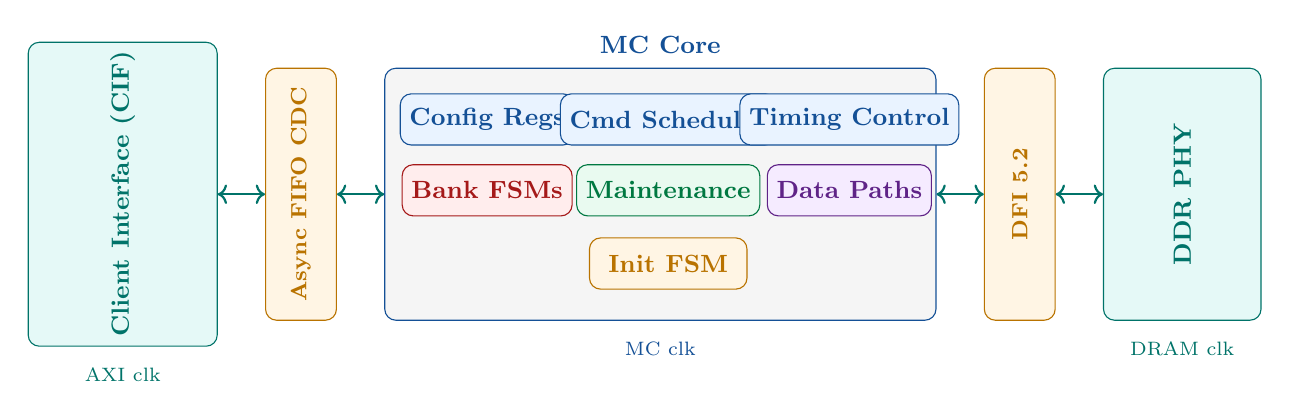
\begin{tikzpicture}[node distance=0.5cm and 0.7cm]
  % CIF domain
  \node[blkteal,minimum width=2.4cm,minimum height=3.2cm](cif)
    {\rotatebox{90}{Client Interface (CIF)}};
  % CDC
  \node[blkamber,right=0.6cm of cif,minimum width=0.9cm,minimum height=3.2cm](cdc)
    {\rotatebox{90}{\footnotesize Async FIFO CDC}};
  % MC Core box
  \node[blk,right=0.6cm of cdc,minimum width=7cm,minimum height=3.2cm,
        fill=rowgray,draw=ddrblue,text=ddrblue](mccore){\phantom{x}};
  \node[above=0.05cm of mccore.north,font=\small\bfseries\color{ddrblue}]{MC Core};
  % inner blocks
  \node[blk,minimum width=2cm,minimum height=0.65cm]
        at ([xshift=-2.2cm,yshift=0.95cm]mccore.center)(cr){Config Regs};
  \node[blk,minimum width=2cm,minimum height=0.65cm]
        at ([xshift=0.1cm,yshift=0.95cm]mccore.center)(sched){Cmd Scheduler};
  \node[blk,minimum width=2cm,minimum height=0.65cm]
        at ([xshift=2.4cm,yshift=0.95cm]mccore.center)(tc){Timing Control};
  \node[blkred,minimum width=2cm,minimum height=0.65cm]
        at ([xshift=-2.2cm,yshift=0.05cm]mccore.center)(bsm){Bank FSMs};
  \node[blkgreen,minimum width=2cm,minimum height=0.65cm]
        at ([xshift=0.1cm,yshift=0.05cm]mccore.center)(maint){Maintenance};
  \node[blkpurple,minimum width=2cm,minimum height=0.65cm]
        at ([xshift=2.4cm,yshift=0.05cm]mccore.center)(dp){Data Paths};
  \node[blkamber,minimum width=2cm,minimum height=0.65cm]
        at ([xshift=0.1cm,yshift=-0.88cm]mccore.center)(init){Init FSM};
  % DFI
  \node[blkamber,right=0.6cm of mccore,minimum width=0.9cm,minimum height=3.2cm](dfi)
    {\rotatebox{90}{\footnotesize DFI 5.2}};
  % PHY
  \node[blkteal,right=0.6cm of dfi,minimum width=2cm,minimum height=3.2cm](phy)
    {\rotatebox{90}{DDR PHY}};

  % Arrows
  \draw[arr,<->](cif.east)--(cdc.west);
  \draw[arr,<->](cdc.east)--(mccore.west);
  \draw[arr,<->](mccore.east)--(dfi.west);
  \draw[arr,<->](dfi.east)--(phy.west);

  % Domain labels
  \node[below=0.15cm of cif,font=\scriptsize,color=ddrteal]{AXI clk};
  \node[below=0.15cm of mccore,font=\scriptsize,color=ddrblue]{MC clk};
  \node[below=0.15cm of phy,font=\scriptsize,color=ddrteal]{DRAM clk};
\end{tikzpicture}
\end{center}

\vspace{1cm}
\begin{tabular}{@{}ll@{}}
  \textbf{Standard}    & JEDEC JESD79-5 (DDR5), DFI 5.2, AXI4 \\[2pt]
  \textbf{Banks}       & 16 (2 BG $\times$ 4 banks, per sub-channel) \\[2pt]
  \textbf{Burst}       & BL16 default (BL/2 = 8 clock cycles) \\[2pt]
  \textbf{Clock}       & Dual domain: AXI (CIF) / MC (DRAM), CDC at one crossing point \\[2pt]
  \textbf{FSMs}        & 23 total: 1 Init + 16 BSM + 4 Maintenance + Scheduler + CRC + ECS \\[2pt]
  \textbf{DFI freq}    & 1:1, 1:2, 1:4 ratio supported \\[2pt]
\end{tabular}
\vfill
{\small\color{gray}Memory Controller Capstone --- JESD79-5 / DFI 5.2 / AXI4}
\end{titlepage}

\tableofcontents\newpage

%% ════════════════════════════════════════════════════════════
\section{System Overview}

The MC Core is the central engine of the Reconfigurable Memory Controller (RMC).
It sits entirely in the MC clock domain, receiving commands from the Client Interface
(CIF) via a single Async FIFO CDC bar, and emitting DFI 5.2 commands toward the
DDR PHY. Every DRAM timing constraint, scheduling decision, refresh housekeeping,
and power-state transition is the MC Core's responsibility.

\subsection{Top-Level Signal Flow}

\begin{center}
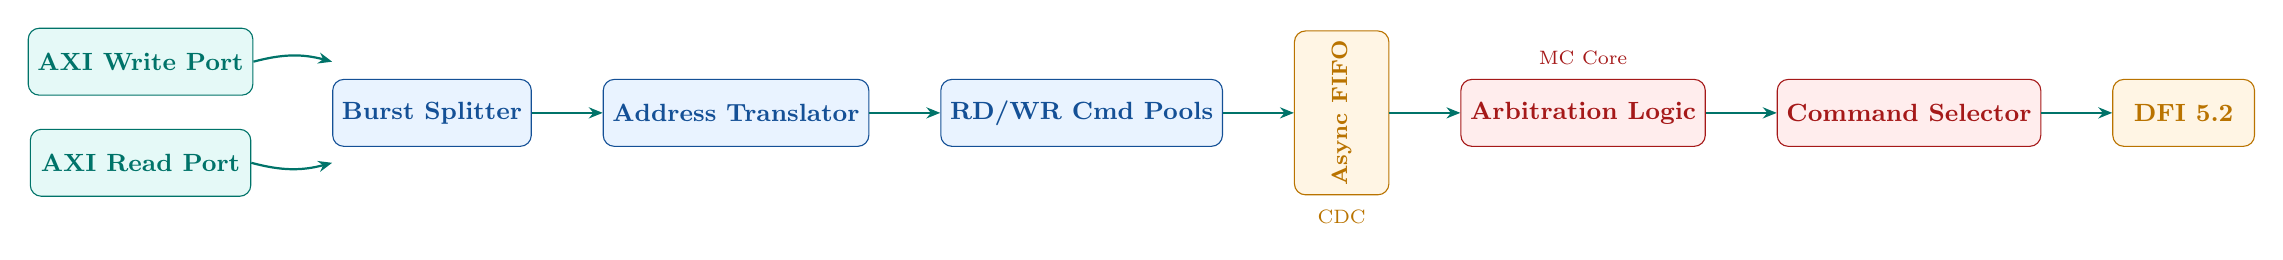
\begin{tikzpicture}[node distance=0.42cm]
  \node[blkteal,minimum width=2.8cm](axi){AXI Write Port};
  \node[blkteal,below=of axi,minimum width=2.8cm](axir){AXI Read Port};
  \node[blk,right=1cm of axi,yshift=-0.65cm,minimum width=2.2cm](bs){Burst Splitter};
  \node[blk,right=0.9cm of bs,minimum width=2.2cm](at){Address Translator};
  \node[blk,right=0.9cm of at,minimum width=2.2cm](pool){RD/WR Cmd Pools};
  \node[blkamber,right=0.9cm of pool,minimum width=1.2cm,minimum height=1.7cm](cdc)
    {\rotatebox{90}{\footnotesize Async FIFO}};
  \node[blkred,right=0.9cm of cdc,minimum width=2.2cm](arb){Arbitration Logic};
  \node[blkred,right=0.9cm of arb,minimum width=2.2cm](sel){Command Selector};
  \node[blkamber,right=0.9cm of sel,minimum width=1.8cm](dfi){DFI 5.2};

  \draw[arr](axi.east)  to[bend left=15]  (bs.west|-axi.east);
  \draw[arr](axir.east) to[bend right=15] (bs.west|-axir.east);
  \draw[arr](bs.east)--(at.west);
  \draw[arr](at.east)--(pool.west);
  \draw[arr](pool.east)--(cdc.west);
  \draw[arr](cdc.east)--(arb.west);
  \draw[arr](arb.east)--(sel.west);
  \draw[arr](sel.east)--(dfi.west);

  \node[below=0.06cm of cdc,font=\scriptsize\color{ddramber}]{CDC};
  \node[above=0.06cm of arb,font=\scriptsize\color{ddrred}]{MC Core};
\end{tikzpicture}
\end{center}

\subsection{Sub-Block Summary}

\begin{longtable}{L{3.4cm} L{2cm} L{9.1cm}}
\toprule
\textbf{Sub-Block} & \textbf{Domain} & \textbf{Role} \\
\midrule
\endfirsthead
\toprule\textbf{Sub-Block}&\textbf{Domain}&\textbf{Role}\\\midrule\endhead
\bottomrule\endfoot

\rowcolor{rowblue}
Config Registers     & MC & Holds all timing knobs, page policy, refresh mode, RFM
                            thresholds, DFI latency offsets. Written via AXI4-Lite CSR path. \\
Init FSM             & MC & Full DDR5 power-up sequence: RESET\_n, NOP burst, DLL reset,
                            ZQcal via MPC, MRW burst, optional training dispatch. Single instance. \\
\rowcolor{rowblue}
Bank State Machines  & MC & 16 instances. Each tracks its bank's state and owns all
                            per-bank timers. Source of truth for bank availability. \\
Timing Control       & MC & Combinational + registered timer array. Produces
                            \sig{cmd\_ok[15:0][cmd\_type]} each cycle for the Scheduler. \\
\rowcolor{rowblue}
Arbitration Logic    & MC & Picks the winner command class each MC clock cycle.
                            Implements priority, age-based anti-starvation, and watermark-controlled
                            RD/WR mode switching. \\
Command Selector     & MC & Takes the winner class, applies all DRAM timing constraints,
                            enforces page policy, emits the final command tuple
                            \{cmd, rank, BG, bank, row, col\}. \\
\rowcolor{rowblue}
Refresh Scheduler    & MC & Leaky-bucket tREFI tracking. REFab and REFsb modes.
                            Handles up to $8\times$ postponement; asserts ref\_urgent on overflow. \\
ZQcal FSM            & MC & Periodic MPC ZQCAL Start/Latch sequence. \\
\rowcolor{rowblue}
RFM FSM              & MC & DDR5 rowhammer mitigation. Per-bank RAA counters;
                            triggers RFM command when RAA $\leq$ RAAIMT. \\
Power Management FSM & MC & CKE-controlled transitions: Active PD, Precharge PD,
                            Self-Refresh, MPSM. \\
\rowcolor{rowblue}
Write Data Path      & MC & BL16-aligned write buffer, DM/ECC generation, Write CRC
                            (CRC-8 over DQ+DM), DFI write timing pipeline. \\
Read Data Path       & MC & Read data capture FIFO, Read CRC/ECC checker,
                            read latency counter, ECS FSM. \\
\end{longtable}

%% ════════════════════════════════════════════════════════════
\section{Config Registers}

All timing parameters consumed by the MC Core live here. The host programs them
before asserting \reg{INIT\_KICK} and may update them at runtime only while the
controller is idle. The scheduler reads timing values combinatorially every cycle.

\begin{longtable}{L{3cm} C{1.5cm} L{9cm}}
\toprule
\textbf{Register} & \textbf{Width} & \textbf{Description} \\
\midrule
\endfirsthead
\toprule\textbf{Register}&\textbf{Width}&\textbf{Description}\\\midrule\endhead
\bottomrule\endfoot

\rowcolor{rowblue}
\reg{CL}            & 7b  & CAS Latency in nCK. Drives RL used in RTW formula. \\
\reg{CWL}           & 7b  & CAS Write Latency = CL$-$2 (fixed in DDR5). \\
\rowcolor{rowblue}
\reg{tRCD}          & 8b  & RAS-to-CAS delay (nCK). ACT to first RD/WR on same bank. \\
\reg{tRP}           & 8b  & Row Precharge Time (nCK). PRE to next ACT on same bank. \\
\rowcolor{rowblue}
\reg{tRAS}          & 9b  & Row Active Time minimum (nCK). ACT to PRE minimum. \\
\reg{tRC}           & 9b  & Row Cycle Time = tRAS+tRP. ACT to ACT same bank. \\
\rowcolor{rowblue}
\reg{tWR}           & 8b  & Write Recovery Time (nCK). WR burst end to PRE. \\
\reg{tRTP}          & 6b  & Read-to-Precharge (nCK). RD cmd to PRE on same bank. \\
\rowcolor{rowblue}
\reg{tCCD\_L}       & 5b  & CAS-to-CAS, same BG (nCK). \\
\reg{tCCD\_S}       & 5b  & CAS-to-CAS, diff BG = BL/2 = 8 nCK. \\
\rowcolor{rowblue}
\reg{tCCD\_L\_WR}   & 6b  & WR-to-WR, same BG (nCK). max(32 nCK, 20 ns) per spec. \\
\reg{tCCD\_L\_WR2}  & 6b  & WR-to-WR, same BG, 2nd not RMW (nCK). max(16 nCK, 10 ns). \\
\rowcolor{rowblue}
\reg{tWTR\_L}       & 6b  & Write-to-Read same BG (nCK). \\
\reg{tWTR\_S}       & 5b  & Write-to-Read diff BG (nCK). \\
\rowcolor{rowblue}
\reg{tRRD\_L}       & 5b  & ACT-to-ACT same BG (nCK). \\
\reg{tRRD\_S}       & 4b  & ACT-to-ACT diff BG (nCK). \\
\rowcolor{rowblue}
\reg{tFAW}          & 6b  & Four-Activate Window (nCK). \\
\reg{tRFC1}         & 12b & REFab recovery time (nCK). 195 ns for 8\,Gb DDR5. \\
\rowcolor{rowblue}
\reg{tRFCsb}        & 11b & REFsb per-bank recovery (nCK). \\
\reg{tREFI}         & 14b & Average refresh interval (nCK). 3.9\,\textmu s at $\leq$85\textdegree C. \\
\rowcolor{rowblue}
\reg{tMRD}          & 5b  & MRW-to-MRW minimum (nCK). 16 nCK in DDR5. \\
\reg{tXP}           & 5b  & PDX-to-command (nCK). \\
\rowcolor{rowblue}
\reg{tXS}           & 12b & SRX-to-command without DLL lock (nCK). tRFC1+10\,ns. \\
\reg{tCKSRE}        & 5b  & Stable clock cycles required after SRE. \\
\rowcolor{rowblue}
\reg{tCKSRX}        & 5b  & Stable clock cycles required before SRX. \\
\reg{tDLLK}         & 11b & DLL lock time after DLL Reset MPC. 1024 nCK. \\
\rowcolor{rowblue}
\reg{RAAIMT}        & 8b  & RFM RAA Initial Management Threshold (from MR58). \\
\reg{RAAMMT}        & 8b  & RFM RAA Maximum Management Threshold (from MR58). \\
\rowcolor{rowblue}
\reg{RAADec}        & 4b  & RAA decrement per REF command issued. \\
\reg{REF\_MODE}     & 2b  & 00=REFab, 01=REFsb, 10=FGR-2x, 11=FGR-4x. \\
\rowcolor{rowblue}
\reg{PAGE\_POLICY}  & 2b  & 00=Open, 01=Closed, 10=Adaptive. \\
\reg{AGE\_THR1}     & 8b  & Intra-class age escalation threshold (cycles). \\
\rowcolor{rowblue}
\reg{AGE\_THR2}     & 8b  & Cross-class age escalation threshold (cycles). \\
\reg{WR\_HIGH\_WM}  & 6b  & Write pool watermark high --- triggers switch to WR mode. \\
\rowcolor{rowblue}
\reg{WR\_LOW\_WM}   & 6b  & Write pool watermark low --- triggers switch back to RD mode. \\
\reg{PHY\_WRLAT}    & 6b  & \sig{dfi\_t\_phy\_wrlat}: WL pipeline offset to PHY. \\
\rowcolor{rowblue}
\reg{PHY\_RDLAT}    & 6b  & \sig{dfi\_t\_rddata\_en}: RL pipeline offset to PHY. \\
\reg{FREQ\_RATIO}   & 2b  & DFI frequency ratio: 00=1:1, 01=1:2, 10=1:4. \\
\rowcolor{rowblue}
\reg{INIT\_KICK}    & 1b  & Write 1 to trigger Init FSM. \\
\reg{SOFT\_RESET}   & 1b  & Synchronous soft-reset of all MC Core FSMs. \\
\end{longtable}

%% ════════════════════════════════════════════════════════════
\section{Init FSM}

\begin{notebox}
\textbf{Reference:} JESD79-5 \S3.3.1 (power-up with stable power) and \S3.3.2 (reset with
stable power). Single instance. Triggered by \reg{INIT\_KICK}. Emits DFI commands directly,
bypassing the Cmd Scheduler. Releases \sig{init\_done} on completion.
\end{notebox}

\subsection{States and Transitions}

\begin{longtable}{L{3.8cm} L{5.5cm} L{5.2cm}}
\toprule
\textbf{State} & \textbf{Action} & \textbf{Exit Condition} \\
\midrule
\endfirsthead
\toprule\textbf{State}&\textbf{Action}&\textbf{Exit}\\\midrule\endhead
\bottomrule\endfoot

\rowcolor{rowblue}
\state{IDLE}
  & Hold RESET\_n=0, CKE=0, CS\_n=0. All DFI outputs deasserted.
  & \reg{INIT\_KICK}=1 \\

\state{ASSERT\_RESET}
  & RESET\_n held LOW. CS\_n held LOW. Load tINIT1 (200\,\textmu s) counter.
  & tINIT1 timer expires \\

\rowcolor{rowblue}
\state{CS\_LOW\_PRE\_DEASSERT}
  & CS\_n held LOW. Count tINIT2 (10\,ns) before releasing RESET\_n.
  & tINIT2 timer expires \\

\state{CS\_LOW\_POST\_DEASSERT}
  & Deassert RESET\_n (HIGH). CS\_n remains LOW. CKE still LOW.
    Count tINIT3 (4\,ms).
  & tINIT3 timer expires \\

\rowcolor{rowblue}
\state{ODT\_SETTLE}
  & Raise CKE. Stable CK already running. Count tINIT4 (2\,\textmu s)
    for ODT and CK settle.
  & tINIT4 timer expires \\

\state{NOP\_BURST}
  & Issue $\geq$3 NOP/DES on DFI. CS\_n driven normally.
  & tINIT5 NOP count satisfied \\

\rowcolor{rowblue}
\state{WAIT\_XPR}
  & Count tXPR = max(5\,nCK, tRFC1+10\,ns) after CS\_n first HIGH.
  & tXPR timer expires \\

\state{MPC\_DLL\_DIVIDER}
  & Issue MPC opcode: DLL Divider Select. Configures tCCD\_L divider via MR13.
  & DFI command accepted \\

\rowcolor{rowblue}
\state{MPC\_DLL\_RESET}
  & Issue MPC opcode: DLL Reset. Required before ZQcal per spec.
  & DFI command accepted \\

\state{ZQCAL\_START}
  & Issue MPC opcode: ZQCAL Start (OP=0x00). Initiates impedance calibration.
  & DFI command accepted \\

\rowcolor{rowblue}
\state{WAIT\_tZQCAL}
  & Wait. DRAM performs internal ZQ calibration.
  & tZQCAL (1\,\textmu s) expires \\

\state{ZQCAL\_LATCH}
  & Issue MPC opcode: ZQCAL Latch (OP=0x01). Captures calibrated driver/ODT codes.
  & DFI command accepted \\

\rowcolor{rowblue}
\state{WAIT\_tZQLAT}
  & Wait tZQLAT = 30\,nCK for latch propagation.
  & tZQLAT timer expires \\

\state{MRW\_BURST}
  & Issue MRW to all required mode registers in order: MR0 (BL, CL), MR2
    (functional modes), MR4 (refresh), MR5 (ODT/DM), MR6 (tWR/tRTP), MR8
    (burst/CRC/preamble), MR32--MR35 (ODT), MR58 (RFM). One MRW per
    tMRD (16\,nCK).
  & All required MRWs issued \\

\rowcolor{rowblue}
\state{TRAINING\_DISPATCH}
  & Optional. Controlled by \reg{TRAIN\_EN} register bits. Dispatches CA training,
    CS training, Write Leveling (MR2 OP[5]=1), and read training (MPC RTP Start)
    sub-sequences via DFI training handshake signals.
  & All enabled training sub-sequences complete, or skipped if \reg{TRAIN\_EN}=0 \\

\state{DONE}
  & Assert \sig{init\_done}. Release Cmd Scheduler from reset.
    Init FSM idles until soft-reset or re-kick.
  & Permanent until \reg{SOFT\_RESET} \\
\end{longtable}

\subsection{MRW Sequence Detail}

The MRW burst programs the following registers in order. Each write is separated by tMRD (16\,nCK).

\begin{longtable}{L{1.8cm} L{12.7cm}}
\toprule
\textbf{Register} & \textbf{Fields Programmed} \\
\midrule
\endfirsthead\toprule\textbf{Reg}&\textbf{Fields}\\\midrule\endhead\bottomrule\endfoot
\rowcolor{rowblue}
MR0  & BL = BL16 (OP[1:0]=00), CL from \reg{CL} config reg (OP[6:2]) \\
MR2  & 2N mode, MPSM, write leveling enable if \reg{TRAIN\_EN}[WL]=1 \\
\rowcolor{rowblue}
MR4  & Refresh rate per temperature; FGR mode if \reg{REF\_MODE}[1]=1 \\
MR5  & RTT PARK, DM enable \\
\rowcolor{rowblue}
MR6  & tWR and tRTP from \reg{tWR}, \reg{tRTP} config regs \\
MR8  & Burst length, preamble mode (2/4 tCK), Write CRC enable, Read CRC enable \\
\rowcolor{rowblue}
MR32 & CK ODT, CS ODT \\
MR33 & CA ODT, DQS RTT PARK \\
\rowcolor{rowblue}
MR34 & RTT PARK, RTT WR \\
MR35 & RTT NOM WR, RTT NOM RD \\
\rowcolor{rowblue}
MR58 & Read-only (RAAIMT, RAAMMT). Init FSM reads via MRR and mirrors to \reg{RAAIMT}/\reg{RAAMMT} config regs. \\
\end{longtable}

%% ════════════════════════════════════════════════════════════
\section{Bank State Machines (BSM)}

\begin{notebox}
16 instances, one per bank (2 BG $\times$ 4 banks $\times$ 2 sub-channels per device, or
4 BG $\times$ 4 banks for x4/x8 devices). Each BSM is independent. It receives commands
from the Cmd Scheduler and \sig{cmd\_ok} enables from Timing Control. All per-bank
timers reside inside the BSM.
\end{notebox}

\subsection{States and Transitions}

\begin{longtable}{L{3cm} L{4.2cm} L{7.3cm}}
\toprule
\textbf{State} & \textbf{Legal Input Commands} & \textbf{Entry / Timer / Exit} \\
\midrule
\endfirsthead
\toprule\textbf{State}&\textbf{Legal Inputs}&\textbf{Entry/Timer/Exit}\\\midrule\endhead
\bottomrule\endfoot

\rowcolor{rowblue}
\state{IDLE}
  & ACT, REFab, REFsb, PDE, SRE, RFM
  & Default state. No timer running. Entered from PRECHARGING when tRP expires,
    from REFRESHING when tRFC expires, or at init. \\

\state{ACTIVATING}
  & None (internal delay)
  & Entered on ACT command. Runs tRCD countdown.
    Transitions to \state{BANK\_ACTIVE} when tRCD expires. \\

\rowcolor{rowblue}
\state{BANK\_ACTIVE}
  & RD, RDA, WR, WRA, PRE, PREA
  & Entered from ACTIVATING. tRAS timer loaded at entry.
    PRE only issued after tRAS satisfied.
    Open row address registered for row-hit detection. \\

\state{READING}
  & BST (truncate to BC8)
  & Entered on RD or RDA command. Bus occupied for CL+BL/2 cycles.
    If RDA: hidden precharge starts internally at tRTP after RD.
    Exits to \state{BANK\_ACTIVE} (no AP) or \state{PRECHARGING} (RDA). \\

\rowcolor{rowblue}
\state{WRITING}
  & BST (truncate to BC8)
  & Entered on WR or WRA command. Bus occupied for CWL+BL/2 cycles.
    If WRA: hidden precharge starts at CWL+BL/2.
    Exits to \state{BANK\_ACTIVE} (no AP) or \state{PRECHARGING} (WRA). \\

\state{PRECHARGING}
  & None (internal delay)
  & Entered on PRE/PREA or at end of RDA/WRA burst. tRP counter loaded.
    Transitions to \state{IDLE} when tRP expires. \\

\rowcolor{rowblue}
\state{REFRESHING\_AB}
  & None
  & Entered when Refresh Scheduler issues REFab. All 16 banks enter this state
    simultaneously. tRFC1 counter loaded. All banks return to \state{IDLE}
    when tRFC1 expires. FGR mode: tRFC2 or tRFC4 used instead. \\

\state{REFRESHING\_SB}
  & None
  & Entered when Refresh Scheduler issues REFsb targeting this bank.
    Only the targeted bank is locked; other banks remain accessible.
    tRFCsb counter loaded. Exits to \state{IDLE} when tRFCsb expires. \\

\rowcolor{rowblue}
\state{POWER\_DOWN}
  & PDX
  & Entered from \state{IDLE} (Precharge PD) or \state{BANK\_ACTIVE} (Active PD)
    when CKE deasserted. tCKE minimum low time enforced.
    Exits to \state{IDLE} or \state{BANK\_ACTIVE} respectively after PDX + tXP. \\

\state{SELF\_REFRESH}
  & SRX
  & Entered from \state{IDLE} (all banks must be precharged first).
    tCKSRE stable clock enforced after entry. Minimum tCKESR in SR.
    On SRX: tCKSRX stable clock required, then tXS before any command. \\

\rowcolor{rowblue}
\state{RFM\_ACTIVE}
  & None
  & Entered when RFM FSM issues an RFM command to this bank (RAA $\leq$ RAAIMT).
    tRFM counter loaded (same duration as tRFC1).
    Exits to \state{IDLE} when tRFM expires. \\
\end{longtable}

\subsection{Per-Bank Timer Table}

\begin{longtable}{L{3.5cm} L{4.5cm} L{6.5cm}}
\toprule
\textbf{Timer} & \textbf{Loaded On} & \textbf{Guards} \\
\midrule
\endfirsthead\toprule\textbf{Timer}&\textbf{Loaded On}&\textbf{Guards}\\\midrule\endhead
\bottomrule\endfoot
\rowcolor{rowblue}
tRCD counter   & ACT issued         & First RD/WR on same bank \\
tRAS counter   & ACT issued         & PRE/PREA on same bank (minimum open) \\
\rowcolor{rowblue}
tRC counter    & ACT issued         & Next ACT on same bank \\
tRP counter    & PRE issued         & Next ACT on same bank \\
\rowcolor{rowblue}
tWR counter    & WR burst end       & PRE on same bank \\
tRTP counter   & RD cmd issued      & PRE on same bank \\
\rowcolor{rowblue}
tRFC1 counter  & REFab issued       & Any command on any bank (all banks blocked) \\
tRFCsb counter & REFsb issued       & Commands to the refreshed bank only \\
\rowcolor{rowblue}
tXS counter    & SRX asserted       & First ACT after self-refresh exit \\
tXP counter    & PDX asserted       & First command after power-down exit \\
\rowcolor{rowblue}
tMRD counter   & MRW issued         & Next MRW command \\
\end{longtable}

%% ════════════════════════════════════════════════════════════
\section{Timing Control}

The Timing Control block is not a state machine. It is a \textbf{combinational and
registered timer array} that produces \sig{cmd\_ok[15:0][CMD\_TYPES]} every MC clock
cycle. The Cmd Scheduler may only issue a command if the corresponding
\sig{cmd\_ok} bit is asserted.

\subsection{Per-Bank Countdown Timers}

Each of the 11 per-bank timers (listed above in \S4.2) is implemented as a
down-counter. When the counter reaches zero the relevant \sig{cmd\_ok} bit
is set. The timers are loaded in the same cycle the triggering command is
issued to DFI.

\subsection{Cross-Bank Constraint Checkers}

\begin{longtable}{L{2.8cm} L{3cm} L{8.7cm}}
\toprule
\textbf{Constraint} & \textbf{Scope} & \textbf{Implementation} \\
\midrule
\endfirsthead\toprule\textbf{Constraint}&\textbf{Scope}&\textbf{Implementation}\\\midrule\endhead
\bottomrule\endfoot

\rowcolor{rowblue}
tRRD\_L
  & Same BG, any bank
  & Timestamp of last ACT in same BG stored. New ACT blocked until
    $T_{\text{now}} - T_{\text{last ACT in BG}} \geq$ tRRD\_L. \\

tRRD\_S
  & Diff BG, any bank
  & Timestamp of last ACT globally. New ACT in a different BG blocked until
    $T_{\text{now}} - T_{\text{last ACT any}} \geq$ tRRD\_S. \\

\rowcolor{rowblue}
tFAW
  & All banks, same rank
  & 4-entry ring buffer of the most recent ACT timestamps.
    New ACT blocked if the oldest of the 4 timestamps is within tFAW cycles.
    \texttt{faw\_ok = (now - act\_ts[3]) $\geq$ tFAW}. \\

tCCD\_L
  & Same BG, RD/WR
  & Timestamp of last CAS in same BG. Next CAS in same BG blocked until
    $\Delta T \geq$ tCCD\_L. For WR-to-WR same BG, tCCD\_L\_WR is used.
    For WR-to-WR same BG when 2nd write is not RMW: tCCD\_L\_WR2. \\

\rowcolor{rowblue}
tCCD\_S
  & Diff BG, RD/WR
  & Timestamp of last CAS globally. Next CAS in different BG blocked until
    $\Delta T \geq$ tCCD\_S (= BL/2 = 8\,nCK in DDR5). \\

tWTR\_L
  & Same BG, WR$\to$RD
  & Timestamp of last write data end in same BG. RD command blocked until
    $\Delta T \geq$ WL + BL/2 + tWTR\_L. \\

\rowcolor{rowblue}
tWTR\_S
  & Diff BG, WR$\to$RD
  & Same but using tWTR\_S. Enforces $\Delta T \geq$ WL + BL/2 + tWTR\_S. \\

tRTW
  & Any, RD$\to$WR
  & Timestamp of last RD command. WR command blocked until
    $\Delta T \geq$ RL + BL/2 $-$ WL + 2 + tWPRE.
    (tWPRE = 2\,tCK default per MR8.) \\
\end{longtable}

%% ════════════════════════════════════════════════════════════
\section{Arbitration Logic}

Runs every MC clock. Answers: \textit{which command class wins this cycle?}
Does not select bank, row, or column --- that is the Command Selector's job.
Outputs: \sig{arb\_winner[2:0]}, \sig{pool\_ptr}, \sig{mode\_state}, \sig{ref\_urgent}.

\subsection{Priority Hierarchy}

\begin{longtable}{C{1.2cm} L{3.8cm} L{4.5cm} L{4cm}}
\toprule
\textbf{Level} & \textbf{Winner} & \textbf{Condition} & \textbf{Effect} \\
\midrule
\endfirsthead\toprule\textbf{Level}&\textbf{Winner}&\textbf{Condition}&\textbf{Effect}\\\midrule\endhead
\bottomrule\endfoot
\rowcolor{rowred}
0 & REF urgent
  & REF credits $\geq 8$, or time since last REF $>$ tREFI$_{\max}$
  & Hard stall --- all RD/WR suppressed \\
\rowcolor{roworange}
1 & REF nominal
  & tREFI countdown reaches zero
  & REF injected; RD/WR deferred \\
\rowcolor{roworange}
2 & ZQ calibration
  & tZQCS interval expires
  & ZQCS after current REF completes \\
\rowcolor{rowblue}
3 & Read
  & RD pool non-empty AND RD mode active
  & Promoted; BG-aware scheduling \\
\rowcolor{rowblue}
4 & Write
  & WR pool non-empty AND WR mode active
  & Batched; watermark-controlled \\
\rowcolor{rowgray}
5 & Scrubber / MRR
  & Background maintenance, idle slot
  & Lowest; pre-emptible \\
\end{longtable}

\subsection{Age Counter Logic (Anti-Starvation)}

Every RD/WR pool entry carries an age counter incremented each MC cycle it
sits unserved.

\begin{itemize}[leftmargin=1.5em,itemsep=2pt]
  \item Age counter $\geq$ \reg{AGE\_THR1} (default 64 cycles):
        entry jumps to head of its class (intra-class HOL bypass).
  \item Age counter $\geq$ \reg{AGE\_THR2} (default 256 cycles):
        WR entry may overtake the RD priority level (cross-class escalation,
        configurable).
  \item Age counter reset to 0 on dispatch.
\end{itemize}

\subsection{RD/WR Mode Switching (Watermark Logic)}

Prevents excessive tWTR/tRTW turnaround penalties by batching reads and
writes into phases.

\begin{itemize}[leftmargin=1.5em,itemsep=2pt]
  \item \textbf{Switch to WR mode:} WR pool depth $\geq$ \reg{WR\_HIGH\_WM}
        (default 32 entries), OR RD pool empty and WR pool non-empty.
  \item \textbf{Switch back to RD mode:} WR pool depth $\leq$ \reg{WR\_LOW\_WM}
        (default 8 entries), OR WR pool empty and RD pool non-empty, OR
        urgent RD due to age escalation.
  \item Hysteresis gap (HIGH $-$ LOW = 24 entries) prevents mode thrashing.
\end{itemize}

\subsection{REF Credit Tracker}

\begin{itemize}[leftmargin=1.5em,itemsep=2pt]
  \item REF credits += 1 every tREFI.
  \item REF credits $-$= 1 on each REF issued.
  \item \sig{ref\_urgent} = (credits $\geq 8$) OR ($\Delta t_{\text{since last REF}} >$
        tREFI$_{\max}$).
  \item JEDEC allows a maximum of 8 postponed refreshes. When \sig{ref\_urgent}
        asserts, arbitration outputs REF unconditionally regardless of pool state.
  \item Temperature derating: at $>$85\textdegree C (detected from MR4 TUF bit),
        tREFI is halved by the Refresh Scheduler before loading into the credit tracker.
\end{itemize}

%% ════════════════════════════════════════════════════════════
\section{Command Selector}

Takes the winner class from Arbitration Logic, applies all remaining DRAM
timing constraints, and emits the fully resolved command:
\{cmd\_type, rank, BG, bank, row, col, ap, wr\_partial\}.

\subsection{Page Policy Engine}

\begin{longtable}{L{3cm} L{4cm} L{7.5cm}}
\toprule
\textbf{Policy} & \textbf{Row Hit} & \textbf{Row Miss / Empty} \\
\midrule
\endfirsthead\toprule\textbf{Policy}&\textbf{Hit}&\textbf{Miss/Empty}\\\midrule\endhead
\bottomrule\endfoot
\rowcolor{rowblue}
Open Page (default)
  & CAS only
  & Miss: PRE $\xrightarrow{\text{tRP}}$ ACT $\xrightarrow{\text{tRCD}}$ CAS.
    Empty: ACT $\xrightarrow{\text{tRCD}}$ CAS. \\
Closed Page
  & ACT + CAS (always)
  & ACT $\xrightarrow{\text{tRCD}}$ CAS.
    Best for random/streaming workloads. \\
\rowcolor{rowblue}
Adaptive
  & Starts as Open
  & Hit-rate tracked over sliding window $N=256$ accesses.
    Hit rate $>$ \reg{OPEN\_THR} (70\%): stay open.
    Hit rate $<$ \reg{CLOSE\_THR} (30\%): switch to closed.
    Autotunes per bank independently. \\
\end{longtable}

\subsection{Bank-Group Aware Reordering}

DDR5 imposes a large same-BG write penalty: tCCD\_L\_WR = max(32\,nCK, 20\,ns)
vs.\ tCCD\_S = 8\,nCK for different BG. The Command Selector scans the candidate
queue for cross-BG entries to exploit the shorter gap. Reordering is bounded
by the age limit to prevent starvation.

\begin{longtable}{L{4.5cm} L{3.5cm} L{3.5cm}}
\toprule
\textbf{Transition} & \textbf{Same BG} & \textbf{Diff BG} \\
\midrule
\endfirsthead\toprule\textbf{Transition}&\textbf{Same BG}&\textbf{Diff BG}\\\midrule\endhead
\bottomrule\endfoot
\rowcolor{rowblue}
RD $\to$ RD    & tCCD\_L = max(8\,nCK, 5\,ns)       & tCCD\_S = 8\,nCK \\
WR $\to$ WR    & tCCD\_L\_WR = max(32\,nCK, 20\,ns) & tCCD\_S = 8\,nCK \\
\rowcolor{rowblue}
WR $\to$ WR (2nd not RMW) & tCCD\_L\_WR2 = max(16\,nCK, 10\,ns) & tCCD\_S \\
\end{longtable}

\subsection{Legal Check Matrix}

Before dispatching any candidate command, all of the following gates must be
true simultaneously. A false on any gate causes a NOP to be inserted that cycle.

\begin{longtable}{L{3.5cm} L{3.5cm} L{7.5cm}}
\toprule
\textbf{Gate} & \textbf{Timer Source} & \textbf{Constraint} \\
\midrule
\endfirsthead\toprule\textbf{Gate}&\textbf{Timer}&\textbf{Constraint}\\\midrule\endhead
\bottomrule\endfoot
\rowcolor{rowblue}
bank\_avail[b]    & BSM state       & Bank not in ACTIVATING or PRECHARGING \\
gate\_rcd[b]      & ACT issue       & tRCD: ACT to first CAS on same bank \\
\rowcolor{rowblue}
gate\_rp[b]       & PRE issue       & tRP: PRE to ACT on same bank \\
gate\_ras[b]      & ACT issue       & tRAS: ACT to PRE minimum \\
\rowcolor{rowblue}
gate\_ccd\_l      & Same BG CAS     & tCCD\_L or tCCD\_L\_WR or tCCD\_L\_WR2 \\
gate\_ccd\_s      & Diff BG CAS     & tCCD\_S = BL/2 \\
\rowcolor{rowblue}
gate\_rrd\_l      & Same BG ACT     & tRRD\_L \\
gate\_rrd\_s      & Diff BG ACT     & tRRD\_S \\
\rowcolor{rowblue}
gate\_faw         & Sliding window  & $\leq 4$ ACTs within tFAW \\
gate\_wtr\_l      & WR data end, same BG & tWTR\_L: WR to RD \\
\rowcolor{rowblue}
gate\_wtr\_s      & WR data end, diff BG & tWTR\_S: WR to RD \\
gate\_rtw         & RD cmd          & tRTW = RL + BL/2 + 2 $-$ WL \\
\rowcolor{rowblue}
gate\_rfc[r]      & REF issue (per rank)    & tRFC1: all commands blocked \\
gate\_rfcpb[r][b] & REFsb (per bank)        & tRFCsb: same bank only blocked \\
\rowcolor{rowblue}
gate\_zqcs        & ZQCS issue      & All commands blocked during ZQ \\
gate\_mrd         & MRW issue       & tMRD: MRW to MRW \\
\end{longtable}

\subsection{Command Sequence Generator}

Outputs into a 4-deep command FIFO. During ACT/PRE wait cycles, other banks
may be serviced (pipelining).

\begin{longtable}{L{3cm} L{11.5cm}}
\toprule
\textbf{Page Decision} & \textbf{Emitted Sequence} \\
\midrule
\endfirsthead\toprule\textbf{Decision}&\textbf{Sequence}\\\midrule\endhead
\bottomrule\endfoot
\rowcolor{rowblue}
Row Hit     & CAS (RD/WR) \\
Row Miss    & PRE $\xrightarrow{\text{tRP}}$ ACT $\xrightarrow{\text{tRCD}}$ CAS \\
\rowcolor{rowblue}
Row Empty   & ACT $\xrightarrow{\text{tRCD}}$ CAS \\
REFab       & REFab $\xrightarrow{\text{tRFC1}}$ NOP$\ldots$ (all banks blocked) \\
\rowcolor{rowblue}
REFsb       & REFsb(bank) $\xrightarrow{\text{tRFCsb}}$ NOP (that bank only; others free) \\
ZQCS        & MPC ZQCAL Start $\xrightarrow{\text{tZQCAL}}$ MPC ZQCAL Latch $\xrightarrow{\text{tZQLAT}}$ ready \\
\rowcolor{rowblue}
MRW         & MRW $\xrightarrow{\text{tMRD}}$ next command \\
\end{longtable}

\subsection{Output Signal Format}

\begin{longtable}{L{3.5cm} C{2cm} L{9cm}}
\toprule
\textbf{Field} & \textbf{Width} & \textbf{Description} \\
\midrule
\endfirsthead\toprule\textbf{Field}&\textbf{Width}&\textbf{Description}\\\midrule\endhead
\bottomrule\endfoot
\rowcolor{rowblue}
cmd\_type   & 3b & ACT / RD / WR / PRE / REF / NOP / MRS / ZQCS \\
rank        & 2b & Target rank \\
\rowcolor{rowblue}
bank\_group & 3b & BG[2:0] for x4/x8; BG[1:0] for x16 \\
bank        & 2b & Bank within BG \\
\rowcolor{rowblue}
row         & 17b & Row address (used in ACT) \\
col         & 11b & Column address (used in CAS) \\
\rowcolor{rowblue}
ap          & 1b & Auto-precharge flag (CA10) \\
wr\_partial & 1b & WR\_PARTIAL: triggers internal RMW path in DRAM \\
\end{longtable}

%% ════════════════════════════════════════════════════════════
\section{Maintenance Engine}

The Maintenance Engine runs four independent sub-FSMs that handle all
autonomous background operations. Each posts requests to the Cmd Scheduler
via a priority request bus.

\subsection{Refresh Scheduler FSM}

\textbf{States:} \state{IDLE} $\to$ \state{REF\_DUE} $\to$ \state{WAIT\_BANKS\_IDLE}
$\to$ \state{ISSUE\_REF} $\to$ \state{WAIT\_tRFC} $\to$ \state{DONE} $\to$
\state{IDLE}.

\textbf{REFsb path} (when \reg{REF\_MODE}=01): \state{REF\_DUE} $\to$
\state{WAIT\_TARGET\_BANK\_IDLE} $\to$ \state{ISSUE\_REFsb} $\to$
\state{WAIT\_tRFCsb} $\to$ \state{DONE} $\to$ \state{IDLE}.

\begin{itemize}[leftmargin=1.5em,itemsep=2pt]
  \item \textbf{Leaky-bucket counter:} increments by 1 each tREFI. On REF
        issued: decrement by 1. If counter reaches 9: \sig{ref\_urgent} asserted,
        hard-stalling all RD/WR.
  \item \textbf{REFsb cycling:} bank address cycles BA[1:0] in order 00$\to$01$\to$10$\to$11.
        8 REFsb commands $\approx$ 1 REFab credit.
  \item \textbf{FGR mode:} when \reg{REF\_MODE}[1]=1, tRFC used is tRFC2;
        when \reg{REF\_MODE}[1:0]=11, tRFC4. Budget counter threshold is
        halved or quartered accordingly.
  \item \textbf{Temperature derating:} if MR4 TUF=1, tREFI is halved before
        loading into the credit tracker. Controller polls MR4 periodically via
        background MRR.
\end{itemize}

\subsection{ZQcal FSM}

\textbf{States:} \state{IDLE} $\to$ \state{WAIT\_IDLE} $\to$
\state{ISSUE\_ZQCAL\_START} $\to$ \state{WAIT\_tZQCAL} $\to$
\state{ISSUE\_ZQCAL\_LATCH} $\to$ \state{WAIT\_tZQLAT} $\to$
\state{DONE} $\to$ \state{IDLE}.

Triggered by: periodic tZQCS interval timer (CSR-configurable), or host
write to \reg{ZQCAL\_TRIG} bit. All banks must be idle before issuing.
During ZQCAL, all commands are blocked via \sig{gate\_zqcs}.

\subsection{RFM FSM (Rowhammer Management)}

\textbf{States:} \state{IDLE} $\to$ \state{MONITOR\_RAA} $\to$
\state{RFM\_REQUEST} $\to$ \state{WAIT\_ISSUE} $\to$
\state{WAIT\_tRFM} $\to$ \state{UPDATE\_RAA} $\to$ \state{MONITOR\_RAA}.

\textbf{RAA counter logic:}
\begin{itemize}[leftmargin=1.5em,itemsep=2pt]
  \item RAA[b] += 1 on every ACT to bank $b$.
  \item RAA[b] $-$= \reg{RAADec} on every REF issued to bank $b$.
  \item When RAA[b] $\leq$ \reg{RAAIMT}: assert RFM request to Scheduler
        (priority: above ZQcal, below refresh override).
  \item tRFM = tRFC1 (same duration). Bank enters \state{RFM\_ACTIVE} during this window.
  \item After tRFM: RAA[b] reset to RAAIMT. Return to \state{MONITOR\_RAA}.
\end{itemize}

\subsection{Power Management FSM}

\textbf{States:}
\state{NORMAL} $\to$ \state{PD\_ENTRY\_CHECK} $\to$
\state{PRECHARGE\_PD} or \state{ACTIVE\_PD} $\to$
\state{PDX\_WAIT\_tXP} $\to$ \state{NORMAL}.

\textbf{Self-Refresh branch:}
\state{NORMAL} $\to$ \state{SR\_ENTRY} $\to$ \state{WAIT\_tCKSRE} $\to$
\state{SELF\_REFRESHING} $\to$ \state{SR\_EXIT} $\to$
\state{WAIT\_tCKSRX} $\to$ \state{WAIT\_tXS} $\to$
\state{WAIT\_tDLLK} $\to$ \state{NORMAL}.

\begin{itemize}[leftmargin=1.5em,itemsep=2pt]
  \item \textbf{Precharge PD:} entered from \state{IDLE}. All banks idle. CKE deasserted.
  \item \textbf{Active PD:} entered from \state{BANK\_ACTIVE}. Bank retains open row.
        On PDX: bank resumes from \state{BANK\_ACTIVE} after tXP.
  \item \textbf{Self-Refresh:} all banks must be precharged first. tCKSRE stable clock
        enforced after CKE falls. On SRX: tCKSRX stable clock, then tXS,
        then tDLLK for commands requiring locked DLL.
  \item \textbf{MPSM:} MR2 OP[1:0]=01. Deeper power state than SR.
        All banks precharged prerequisite. Exit via DES then MRW to clear MPSM.
\end{itemize}

%% ════════════════════════════════════════════════════════════
\section{Write Data Path}

\begin{longtable}{L{3.6cm} L{10.9cm}}
\toprule
\textbf{Sub-Block} & \textbf{Description} \\
\midrule
\endfirsthead\toprule\textbf{Sub-Block}&\textbf{Description}\\\midrule\endhead
\bottomrule\endfoot

\rowcolor{rowblue}
Write Data Buffer
  & BL16-aligned FIFO. Stores write data arriving from the CIF Write Cmd Pool
    via the CDC FIFO. Dequeued when the Cmd Scheduler confirms a write slot. \\
DM/ECC Generator
  & Computes per-byte Data Mask. Generates inline Write CRC using CRC-8
    polynomial $G(x)=x^4+x+1$ over DQ and DM bits per BL16 burst.
    Write CRC enabled via MR8 OP[6]=1. \\
\rowcolor{rowblue}
WL Align
  & Inserts a programmable pipeline delay equal to CWL nCK to align the
    DQS preamble to the DFI \sig{dfi\_wrdata\_en} assertion.
    Offset loaded from \reg{PHY\_WRLAT} config reg. \\
DFI Write Timing
  & Drives \sig{dfi\_wrdata[127:0]}, \sig{dfi\_wrdata\_mask[15:0]},
    \sig{dfi\_wrdata\_cs\_n}, and \sig{dfi\_parity\_in}.
    Write preamble per MR8 (2\,tCK default, 4\,tCK optional).
    ODT timing via tODTon = WL$-$2 and tODToff = WL+BL/2. \\
\rowcolor{rowblue}
Write CRC Error FSM
  & Monitors \sig{dfi\_alert\_n} from PHY. States:
    \state{NORMAL} $\to$ \state{CRC\_ERROR\_DETECTED} $\to$
    \state{RETRY\_WRITE} $\to$ \state{AUTO\_DISABLE}.
    Retries up to $n$ times (threshold from MR51/52).
    If retry count exceeded: auto-disables Write CRC via MRW to MR8,
    flags error to CIF error register. \\
\end{longtable}

%% ════════════════════════════════════════════════════════════
\section{Read Data Path}

\begin{longtable}{L{3.6cm} L{10.9cm}}
\toprule
\textbf{Sub-Block} & \textbf{Description} \\
\midrule
\endfirsthead\toprule\textbf{Sub-Block}&\textbf{Description}\\\midrule\endhead
\bottomrule\endfoot

\rowcolor{rowblue}
Read Latency Counter
  & Per-outstanding-read counter. Tracks CL + read preamble cycles from
    the RD command issue to expected data arrival on DFI.
    Issues \sig{dfi\_rddata\_en} exactly \reg{PHY\_RDLAT} cycles before
    the expected \sig{dfi\_rddata\_valid}. \\
Read Data FIFO
  & Captures \sig{dfi\_rddata[127:0]} when \sig{dfi\_rddata\_valid} asserts.
    Re-aligns per-burst data and feeds the CIF Reorder Buffer.
    Tags read data with the AXI transaction ID for out-of-order return. \\
\rowcolor{rowblue}
ECC/CRC Checker
  & Verifies Read CRC when MR8 OP[7]=1.
    On CRC error: flags to CIF error register, optionally triggers read
    retry. Read CRC adds a latency adder to RL (Table 365 of JESD79-5). \\
ECS FSM
  & States: \state{IDLE} $\to$ \state{ECS\_ACTIVE} $\to$
    \state{WAIT\_tECS} $\to$ \state{IDLE}.
    Triggered by MR14 (auto-ECS mode) or host MPC request.
    DRAM scrubs its on-die ECC array during tECS window ($\leq$ tRFC1).
    Error logs readable from MR16--MR20. \\
\end{longtable}

%% ════════════════════════════════════════════════════════════
\section{DFI 5.2 Interface}

\begin{notebox}
\textbf{DFI timing:} \sig{dfi\_wrdata\_en} must be asserted \reg{PHY\_WRLAT} cycles
before write data. \sig{dfi\_rddata\_valid} arrives \reg{PHY\_RDLAT} cycles after
the RD command. Both offsets are PHY-specific and set during DFI training.
Frequency ratio (\reg{FREQ\_RATIO}) determines how many nCK per DFI clock.
\end{notebox}

\begin{longtable}{L{4.8cm} C{2.2cm} L{7.5cm}}
\toprule
\textbf{Signal} & \textbf{Direction} & \textbf{Description} \\
\midrule
\endfirsthead\toprule\textbf{Signal}&\textbf{Dir}&\textbf{Description}\\\midrule\endhead
\bottomrule\endfoot

\rowcolor{rowblue}
\sig{dfi\_address[13:0]}     & MC$\to$PHY & CA bus. 2-cycle encoding for DDR5 ACT. \\
\sig{dfi\_cs\_n[1:0]}        & MC$\to$PHY & Chip select per rank. \\
\rowcolor{rowblue}
\sig{dfi\_cke[1:0]}          & MC$\to$PHY & Clock Enable per rank. \\
\sig{dfi\_odt[1:0]}          & MC$\to$PHY & On-Die Termination control per rank. \\
\rowcolor{rowblue}
\sig{dfi\_reset\_n}          & MC$\to$PHY & DRAM RESET\_n driven by Init FSM. \\
\sig{dfi\_act\_n}            & MC$\to$PHY & Activate indicator (DDR5). \\
\rowcolor{rowblue}
\sig{dfi\_bank[1:0]}         & MC$\to$PHY & Bank address. \\
\sig{dfi\_bg[2:0]}           & MC$\to$PHY & Bank group (BG[2:0] x4/x8; BG[1:0] x16). \\
\rowcolor{rowblue}
\sig{dfi\_wrdata[127:0]}     & MC$\to$PHY & Write data bus (BL16 $\times$ DQ8 per sub-channel). \\
\sig{dfi\_wrdata\_mask[15:0]}& MC$\to$PHY & Write data mask per byte lane. \\
\rowcolor{rowblue}
\sig{dfi\_wrdata\_en}        & MC$\to$PHY & Write data enable. Asserted \reg{PHY\_WRLAT} cycles early. \\
\sig{dfi\_wrdata\_cs\_n}     & MC$\to$PHY & Per-DRAM write chip select (DDR5 PDA). \\
\rowcolor{rowblue}
\sig{dfi\_parity\_in}        & MC$\to$PHY & CA parity bit (DDR5). \\
\sig{dfi\_rddata[127:0]}     & PHY$\to$MC & Captured read data from PHY. \\
\rowcolor{rowblue}
\sig{dfi\_rddata\_valid}     & PHY$\to$MC & Read data valid. Read Data FIFO captures on this. \\
\sig{dfi\_rddata\_dnv}       & PHY$\to$MC & Data-not-valid error flag. \\
\rowcolor{rowblue}
\sig{dfi\_alert\_n}          & PHY$\to$MC & DRAM alert: Write CRC error or CA parity error. \\
\sig{dfi\_ctrlupd\_req}      & MC$\to$PHY & Controller requests PHY update (periodic). \\
\rowcolor{rowblue}
\sig{dfi\_ctrlupd\_ack}      & PHY$\to$MC & PHY acknowledges update request. \\
\sig{dfi\_phyupd\_req}       & PHY$\to$MC & PHY requests MC to pause command issue. \\
\rowcolor{rowblue}
\sig{dfi\_phyupd\_ack}       & MC$\to$PHY & MC acknowledges PHY update pause. \\
\sig{dfi\_init\_start}       & MC$\to$PHY & Init FSM: start PHY initialization handshake. \\
\rowcolor{rowblue}
\sig{dfi\_init\_complete}    & PHY$\to$MC & PHY initialization done. \\
\sig{dfi\_freq\_ratio[1:0]}  & MC$\to$PHY & Frequency ratio: 00=1:1, 01=1:2, 10=1:4. \\
\end{longtable}

%% ════════════════════════════════════════════════════════════
\section{FSM Inventory}

\begin{longtable}{L{4.2cm} C{2cm} C{2.2cm} L{6.1cm}}
\toprule
\textbf{FSM} & \textbf{States} & \textbf{Instances} & \textbf{Notes} \\
\midrule
\endfirsthead\toprule\textbf{FSM}&\textbf{States}&\textbf{Instances}&\textbf{Notes}\\\midrule\endhead
\bottomrule\endfoot

\rowcolor{rowblue}
Init FSM              & 16 & 1  & Longest chain; RESET\_n through training complete \\
Bank State Machine    & 11 & 16 & One per bank; 176 total state bits \\
\rowcolor{rowblue}
Arbitration Logic     & 6  & 1  & RD/WR mode + priority selection \\
Command Selector      & 4  & 1  & Page policy + legal check + sequence gen \\
\rowcolor{rowblue}
Refresh Scheduler     & 7  & 1  & REFab + REFsb + FGR + urgent override \\
ZQcal FSM             & 7  & 1  & MPC ZQCAL Start/Latch flow \\
\rowcolor{rowblue}
RFM FSM               & 6  & 1  & Per-bank RAA monitoring + RFM injection \\
Power Management FSM  & 10 & 1  & PD (Pre/Act), SR, MPSM \\
\rowcolor{rowblue}
Write CRC Error FSM   & 4  & 1  & dfi\_alert\_n monitoring; retry + auto-disable \\
ECS FSM               & 4  & 1  & DDR5 inline ECC scrub window \\
\midrule
\rowcolor{lightgray}
\textbf{Total}        & \textbf{$\approx$75} & \textbf{23} & \\
\end{longtable}

%% ════════════════════════════════════════════════════════════
\section{Timing Reference}

All values at @200\,MHz (tCK=5\,ns, CL=3, CWL=1, BL/2=8) and @100\,MHz (tCK=10\,ns).
These are the simulation-corner reference values used during design verification.
Production values are set via Config Regs based on actual speed bin.

\begin{longtable}{L{4.5cm} L{5.8cm} C{1.8cm} C{1.8cm}}
\toprule
\textbf{Command Sequence} & \textbf{Formula} & \textbf{@200} & \textbf{@100} \\
\midrule
\endfirsthead\toprule\textbf{Sequence}&\textbf{Formula}&\textbf{@200}&\textbf{@100}\\\midrule\endhead
\bottomrule\endfoot

\rowcolor{rowblue}
ACT $\to$ RD/WR (same bank)     & tRCD                          & 4  & 4 \\
ACT $\to$ PRE (same bank, min)  & tRAS                          & 7  & 4 \\
\rowcolor{rowblue}
PRE $\to$ ACT (same bank)       & tRP                           & 4  & 4 \\
ACT $\to$ ACT (same bank)       & tRC = tRAS+tRP                & 11 & 8 \\
\rowcolor{rowblue}
ACT $\to$ ACT (same BG)         & tRRD\_L                       & 4  & 4 \\
ACT $\to$ ACT (diff BG)         & tRRD\_S                       & 2  & 2 \\
\rowcolor{rowblue}
RD $\to$ RD (same BG)           & tCCD\_L                       & 8  & 8 \\
WR $\to$ WR (same BG)           & tCCD\_L\_WR                   & 32 & 32 \\
\rowcolor{rowblue}
WR $\to$ WR same BG (not RMW)   & tCCD\_L\_WR2                  & 16 & 16 \\
RD/WR (diff BG)                 & tCCD\_S = BL/2                & 8  & 8 \\
\rowcolor{rowblue}
RD $\to$ WR (any)               & RL+BL/2$-$WL+2+tWPRE         & 14 & 14 \\
WR $\to$ RD (same BG)           & WL+BL/2+tWTR\_L               & 13 & 13 \\
\rowcolor{rowblue}
WR $\to$ RD (diff BG)           & WL+BL/2+tWTR\_S               & 11 & 11 \\
RD $\to$ PRE (same bank)        & tRTP                          & 4  & 4 \\
\rowcolor{rowblue}
WR $\to$ PRE (same bank)        & CWL+BL/2+tWR                  & 15 & 12 \\
WRA $\to$ ACT (same bank)       & CWL+BL/2+tWR+tRP              & 19 & 16 \\
\rowcolor{rowblue}
RDA $\to$ ACT (same bank)       & tRTP+tRP                      & 8  & 8 \\
REFab $\to$ any                 & tRFC1                         & 39 & 20 \\
\rowcolor{rowblue}
SRX $\to$ ACT (no DLL)          & tXS = tRFC1+10\,ns            & 41 & 21 \\
PDX $\to$ any                   & tXP                           & 5  & 5 \\
\rowcolor{rowblue}
MRW $\to$ MRW                   & tMRD                          & 16 & 16 \\
ZQCAL Start $\to$ Latch         & tZQCAL = 1\,\textmu s         & 200 & 100 \\
\rowcolor{rowblue}
ZQCAL Latch $\to$ next cmd      & tZQLAT                        & 30 & 30 \\
4 ACT window                    & tFAW                          & 16 & 16 \\
\end{longtable}

%% ════════════════════════════════════════════════════════════
\section{Constraint Support Checklist}

\begin{longtable}{L{6cm} C{1.5cm} L{7cm}}
\toprule
\textbf{Constraint} & \textbf{Status} & \textbf{Notes} \\
\midrule
\endfirsthead\toprule\textbf{Constraint}&\textbf{Status}&\textbf{Notes}\\\midrule\endhead
\bottomrule\endfoot

\multicolumn{3}{l}{\small\textbf{CAS-to-CAS}} \\[2pt]
\rowcolor{rowblue}
tCCD\_L same BG RD$\to$RD    & \yes & max(8\,nCK, 5\,ns); BG tracker \\
tCCD\_S diff BG RD$\to$RD    & \yes & 8\,nCK \\
\rowcolor{rowblue}
tCCD\_L\_WR same BG WR$\to$WR & \yes & max(32\,nCK, 20\,ns) \\
tCCD\_L\_WR2 same BG WR$\to$WR (2nd not RMW) & \yes & max(16\,nCK, 10\,ns) \\
\rowcolor{rowblue}
tCCD\_S\_WR diff BG WR$\to$WR & \yes & = tCCD\_S = 8\,nCK \\[4pt]

\multicolumn{3}{l}{\small\textbf{ACT-to-ACT}} \\[2pt]
\rowcolor{rowblue}
tRRD\_L same BG               & \yes & max(8\,nCK, 5\,ns) \\
tRRD\_S diff BG               & \yes & 8\,nCK \\
\rowcolor{rowblue}
tRRD\_L(1K) / tRRD\_L(2K)    & \yes & 1\,KB and 2\,KB page size differentiation \\
tFAW 4-ACT window             & \yes & 4-entry shift register of ACT timestamps \\[4pt]

\rowcolor{rowblue}
\multicolumn{3}{l}{\small\textbf{ACT / PRE / Row Timing}} \\[2pt]
tRCD, tRP, tRAS               & \yes & Per-bank countdown timers \\
\rowcolor{rowblue}
tRC = tRAS+tRP                & \yes & Implicit from tRAS + tRP timers \\
tRTP, tWR                     & \yes & Per-bank timers \\
\rowcolor{rowblue}
tRAS max (row open timeout)   & \no  & Force-PRE on $9\times$tREFI not implemented \\[4pt]

\multicolumn{3}{l}{\small\textbf{Write/Read Turnaround}} \\[2pt]
\rowcolor{rowblue}
tWTR\_L same BG               & \yes & WL+BL/2+tWTR\_L \\
tWTR\_S diff BG               & \yes & WL+BL/2+tWTR\_S \\
\rowcolor{rowblue}
tRTW                          & \yes & RL+BL/2$-$WL+2 \\[4pt]

\multicolumn{3}{l}{\small\textbf{Refresh}} \\[2pt]
\rowcolor{rowblue}
tRFC1 REFab recovery          & \yes & Per-rank block via gate\_rfc \\
tRFCsb REFsb per-bank         & \yes & Only target bank blocked \\
\rowcolor{rowblue}
tREFI tracking                & \yes & Leaky-bucket; up to 8 postponements \\
ref\_urgent hard stall        & \yes & Asserted at credit = 8 \\
\rowcolor{rowblue}
tREFI derating ($>$85\textdegree C) & \yes & 2$\times$ via MR4 TUF polling \\
Per-bank REFsb credit balance & \no  & Global credit only; per-bank balance not tracked \\
\rowcolor{rowblue}
Automatic BA cycling REFsb    & \no  & BA rotation not enforced in hardware \\
FGR 4$\times$ mode            & \no  & FGR 2$\times$ supported; 4$\times$ not \\[4pt]

\multicolumn{3}{l}{\small\textbf{ZQ Calibration}} \\[2pt]
\rowcolor{rowblue}
tZQCAL, tZQLAT               & \yes & MPC ZQCAL Start/Latch \\
Periodic tZQCS               & \yes & CSR-configurable interval \\[4pt]

\multicolumn{3}{l}{\small\textbf{Mode Registers}} \\[2pt]
\rowcolor{rowblue}
tMRD (MRW$\to$MRW)           & \yes & \\
tRFC1 ODT: tODTon/tODToff    & \yes & WL$-$2 / WL+BL/2 \\
\rowcolor{rowblue}
Dynamic RTT switching         & \no  & Static RTT programming only \\[4pt]

\multicolumn{3}{l}{\small\textbf{DFI Latency}} \\[2pt]
\rowcolor{rowblue}
dfi\_t\_rddata\_en            & \yes & RL cycles ahead of CAS \\
dfi\_t\_phy\_wrlat            & \yes & WL cycles ahead of data \\
\rowcolor{rowblue}
dfi\_freq\_ratio 1:1/1:2/1:4 & \yes & \\
Read CRC RL adder             & \no  & Not pipelined \\[4pt]

\multicolumn{3}{l}{\small\textbf{Power / Self-Refresh}} \\[2pt]
\rowcolor{rowblue}
tCKSRX, tXS                  & \yes & Init FSM + Power Mgmt FSM \\
MPSM entry/exit              & \no  & All-banks-precharged prerequisite not enforced \\
\rowcolor{rowblue}
Power-down entry/exit        & \no  & Dynamic power-down not supported \\[4pt]

\multicolumn{3}{l}{\small\textbf{RFM / Rowhammer}} \\[2pt]
\rowcolor{rowblue}
RAA counter per bank         & \yes & RFM FSM tracks per-bank RAA \\
RAAIMT threshold monitoring  & \yes & From MR58 mirrored to config reg \\
\rowcolor{rowblue}
RFMab injection              & \yes & Via Maintenance Engine priority request \\
RFMsb injection              & \no  & Not implemented \\
\rowcolor{rowblue}
ALERT\_n RFM decode          & \no  & \\[4pt]

\multicolumn{3}{l}{\small\textbf{Multi-Rank}} \\[2pt]
\rowcolor{rowblue}
Per-rank tRFC isolation      & \yes & gate\_rfc[r] per rank \\
tRRD across ranks            & \yes & \\
\rowcolor{rowblue}
Rank interleave during tRFC  & \yes & Other rank serviced during tRFC bubble \\[4pt]

\multicolumn{3}{l}{\small\textbf{Not Supported / Deferred}} \\[2pt]
\rowcolor{rowred}
tRASmax / force-PRE timeout  & \no  & \\
BL32 timing adjustments      & \no  & \\
\rowcolor{rowred}
2N mode CA pipeline          & \no  & \\
PPR sequence                 & \no  & Guard key + hPPR/sPPR flow \\
\rowcolor{rowred}
ECS scrub address walking    & \no  & MR14--MR21 scrub scheduling \\
DQS oscillator scheduling    & \no  & Post-init re-cal trigger \\
\rowcolor{rowred}
CA parity retry              & \no  & ALERT\_n decode + retransmit \\
Write Pattern command (WRP)  & \no  & \\
\end{longtable}

\begin{center}
{\small\color{gray}
\textbf{Supported: 51} \quad \textbf{Not Supported / Deferred: 27} \quad \textbf{Total: 78}
}
\end{center}

%% ════════════════════════════════════════════════════════════
\section{DDR5 vs DDR4 --- Design Deltas}

\begin{longtable}{L{3.5cm} L{4cm} L{7cm}}
\toprule
\textbf{Feature} & \textbf{DDR4} & \textbf{DDR5 --- MC Core Impact} \\
\midrule
\endfirsthead\toprule\textbf{Feature}&\textbf{DDR4}&\textbf{DDR5}\\\midrule\endhead
\bottomrule\endfoot

\rowcolor{rowblue}
BL             & BL8 (BL/2=4)         & BL16 (BL/2=8). All RTW, WTR, WR-to-PRE
                                         formulae scale by 2. \\
ACT encoding   & 1-cycle CA            & 2-cycle CA. Scheduler must drive CA on two
                                         consecutive rising edges. \\
\rowcolor{rowblue}
REFsb          & Not supported         & Refresh Scheduler adds REFsb path;
                                         per-bank tRFCsb timer in BSM. \\
RFM            & Not supported         & Full RFM FSM; per-bank RAA counters;
                                         RAAIMT/RAAMMT in Config Regs. \\
\rowcolor{rowblue}
ZQ mechanism   & ZQCL/ZQCS commands    & MPC ZQCAL Start+Latch.
                                         Init FSM restructured; ZQcal FSM uses MPC. \\
tRFC1 (8\,Gb) & 350\,ns               & 195\,ns. Shorter penalty; more scheduling headroom. \\
\rowcolor{rowblue}
tREFI          & 7.8\,\textmu s        & 3.9\,\textmu s. Double refresh rate;
                                         budget counter threshold halved. \\
CWL            & Separate lookup table & CWL = CL$-$2 (fixed). Simplifies Config Reg
                                         and RTW formula. \\
\rowcolor{rowblue}
tMOD           & 24\,nCK after any MRS & Replaced by tMRD only (16\,nCK).
                                         No separate tMOD path needed in Scheduler. \\
tCCD\_L\_WR    & Not defined           & max(32\,nCK, 20\,ns). New gate in Command Selector. \\
\rowcolor{rowblue}
Write CRC      & Optional (MR5)        & Mandatory architecture support.
                                         dfi\_alert\_n monitoring; Write CRC Error FSM required. \\
ECS            & Not supported         & ECS FSM in Read Data Path;
                                         hooks into tRFC window; MR14--MR20 support. \\
\rowcolor{rowblue}
MR addressing  & 3 MRs (MR0/1/2/3)    & 256 MRs (MR0--MR255) via MRW/MRR commands.
                                         Init FSM MRW burst extended. \\
\end{longtable}

%% ════════════════════════════════════════════════════════════
\vfill
\begin{center}
\small\textcolor{gray}{%
MC Core Design Specification ---
Memory Controller Capstone Project\\
JEDEC JESD79-5 (DDR5) / DFI 5.2 / AXI4
}
\end{center}

\end{document}
